% Track 1: harness identification (owner of 1c: C; 1a: A; 1b: B). Numbers from harness/hypotheses.md
% (H1 steps 1-3, H2 steps 1-2, H3 steps 1-2).

\section{Which Agent? Harness Identification}
\label{sec:harness}

\paragraph{Classifier.} We train an Extra Trees classifier on per-request features from four groups:
TLS (JA4 and its parts, JA3, cipher and extension counts and order, groups, signature algorithms,
ALPN), HTTP (version, header order and set, User-Agent, Accept, Accept-Encoding), HTTP/2 (the
Akamai-style fingerprint and its parts) and timing. Two timing features use the whole run: the slowest
gap between consecutive requests, and the gap before the first submit. They score a finished visit
rather than a request as it arrives. All results use 5-fold cross-validation grouped by run, so no
visit is split between training and test, and the classifier reports probabilities.

\paragraph{Scripts alone.} On one Linux machine the 12 baseline stacks each kept one JA4 across all
their runs, but shared only 7 JA4s: the four Node stacks built on \texttt{https} share one, Go net/http
and Colly share one, httpx and aiohttp share one. TLS alone reaches a macro F1 of 0.48, every error
inside a shared-JA4 group; the TLS layer identifies the runtime, not the tool. Headers separate the
stacks: macro F1 1.00 with the User-Agent, and 0.89 without it, the only remaining confusion being two
versions of axios.

\paragraph{Agents against scripts (H1).} Claude Code's built-in fetch tool, WebFetch, is its own client.
It sends the User-Agent \texttt{Claude-User} followed by its version and an Accept header that asks for Markdown
first, and its JA4 (\texttt{t13d181000\_...}) matches none of our baselines, the Node stacks included.
It is identical on Linux and Windows. The picture changes when the agent shells out. Given a shell,
Claude Code fetched with curl in 6 of 7 headless runs on Linux and in all 6 on Windows, and Codex used
curl on Linux. Those requests match plain curl on the same machine at every TLS and HTTP/2 field and,
for the page fetch, at the header layer too; the submit differed only in the command the model wrote
(a multipart body in 5 runs, an added Cookie header for Codex). On Windows, 10 of Claude Code's 12
curl requests were labelled as the matching curl script, and agent against script curl scored a macro
F1 of 0.50, chance. H1 therefore holds for agents that shell out, on both systems, and fails for
agents with their own client.

\begin{figure}[t]
  \centering
  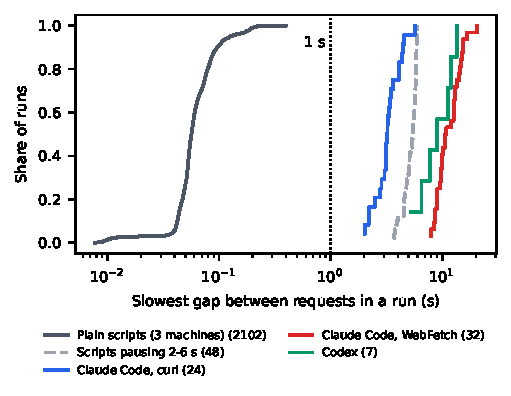
\includegraphics[width=\columnwidth]{figures/timing.pdf}
  \caption{Slowest gap between consecutive requests of each run (cumulative share, log scale). Plain
  scripts on three machines (Linux and two Windows) stay below 0.4\,s; every agent run is above 2\,s.
  Scripts that pause 2 to 6\,s between requests overlap the agents. ``WebFetch'' counts every Claude Code
  run that used WebFetch for at least one request.}
  \label{fig:timing}
\end{figure}

\paragraph{Timing (H2).} What separates an agent's curl from a script's curl is the model in the loop (Figure~\ref{fig:timing}).
A script moves from the page to the submit in milliseconds: on Linux the median gap is 0.005\,s and
the slowest gap in any of 722 runs is 0.105\,s, and no script run on any of the three machines has a
gap above 1\,s. Claude Code with curl waits 3.1 to 3.6\,s, with WebFetch 7.9 to
12.9\,s, and Codex 5.2\,s; a person typing curl took 136\,s. A threshold of 1\,s on the slowest gap
flags all 27 agent runs and none of the 2,102 script runs; on Windows the timing features alone
separate the agent from its script twin with macro F1 1.00, and a timing model trained on one machine
transfers to the other while the TLS features do not. The bound is weak in one direction: a script that
pauses like an agent (2 to 6\,s between requests) is flagged as an agent in all 48 of our runs. Timing
thus separates an LLM in the loop from an automated script, not an agent from a deliberately slowed
script or from a human, and its value for a site depends on the base rate. With no false positive in
2,102 runs, the 95\% upper bound on the false-positive rate is 0.14\%; with recall at least 0.89, a flag
is right at least 38\% of the time when 0.1\% of a site's curl visitors are agents, 86\% at 1\%, and
99\% at 10\%.

\paragraph{The model tier in the trace (H3).} The model also decides which tool fetches the page, and
the tool decides the fingerprint. With WebFetch and a shell both allowed, Haiku read and submitted with
WebFetch in all 12 of its runs; Sonnet read with WebFetch and submitted with curl in 6 of 12 runs and
used curl for both in the other 6; Opus used curl for both in 18 of 19 runs. The sequence of client
fingerprints therefore points to the tier without any text: WebFetch twice is Haiku, WebFetch then curl
is most likely Sonnet. The pause before submitting adds less than it first appeared. On one machine
and day Sonnet's curl submits (2.0 to 2.8\,s) and Opus's (2.9 to 3.6\,s) did not overlap, but Opus
paused 4.1 to 5.7\,s on the same Windows machine a day later, in runs interleaved with the other
models. The pause measures provider-side latency, which drifts, so it can rank models seen in the same
period but not identify one from a fixed threshold.

% TODO (C): add the Codex-on-Windows observation from #39 here or in Section linking: Codex fell back
% from PowerShell and curl to the first Python on PATH, a plain-script fingerprint whose library versions
% are the agent's environment, not the user's.
